\documentclass[11pt, a4paper]{article}
\usepackage{pdfpages}
\usepackage{parallel}
\usepackage[T2A]{fontenc}
\usepackage{ucs}
\usepackage[utf8x]{inputenc}
\usepackage[polish,english,russian]{babel}
\usepackage{hyperref}
\usepackage{rotating}
\usepackage[inner=2cm,top=1.8cm,outer=2cm,bottom=2.3cm,nohead]{geometry}
\usepackage{listings}
\usepackage{graphicx}
\usepackage{wrapfig}
\usepackage{longtable}
\usepackage{indentfirst}
\usepackage{array}
\usepackage{tikzsymbols}
\usepackage{soul}
\usepackage[ruled,vlined]{algorithm2e}
%\counterwithout{figure}{section} 

\usepackage{url}
\makeatletter
\g@addto@macro{\UrlBreaks}{\UrlOrds}
\makeatother

\newcolumntype{P}[1]{>{\raggedright\arraybackslash}p{#1}}
\frenchspacing
\usepackage{fixltx2e} %text sub- and superscripts
\usepackage{icomma} % коскі ў матэматычным рэжыме
\PreloadUnicodePage{4}

\newcommand{\longpage}{\enlargethispage{\baselineskip}}
\newcommand{\shortpage}{\enlargethispage{-\baselineskip}}

\def\switchlang#1{\expandafter\csname switchlang#1\endcsname}
\def\switchlangbe{
\let\saverefname=\refname%
\def\refname{Літаратура}%
\def\figurename{Іл.}%
}
\def\switchlangen{
\let\saverefname=\refname%
\def\refname{References}%
\def\figurename{Fig.}%
}
\def\switchlangru{
\let\saverefname=\refname%
\let\savefigurename=\figurename%
\def\refname{Литература}%
\def\figurename{Рис.}%
}

\hyphenation{admi-ni-stra-tive}
\hyphenation{ex-pe-ri-ence}
\hyphenation{fle-xi-bi-li-ty}
\hyphenation{Py-thon}
\hyphenation{ma-the-ma-ti-cal}
\hyphenation{re-ported}
\hyphenation{imp-le-menta-tions}
\hyphenation{pro-vides}
\hyphenation{en-gi-neering}
\hyphenation{com-pa-ti-bi-li-ty}
\hyphenation{im-pos-sible}
\hyphenation{desk-top}
\hyphenation{elec-tro-nic}
\hyphenation{com-pa-ny}
\hyphenation{de-ve-lop-ment}
\hyphenation{de-ve-loping}
\hyphenation{de-ve-lop}
\hyphenation{da-ta-ba-se}
\hyphenation{plat-forms}
\hyphenation{or-ga-ni-za-tion}
\hyphenation{pro-gramming}
\hyphenation{in-stru-ments}
\hyphenation{Li-nux}
\hyphenation{sour-ce}
\hyphenation{en-vi-ron-ment}
\hyphenation{Te-le-pathy}
\hyphenation{Li-nux-ov-ka}
\hyphenation{Open-BSD}
\hyphenation{Free-BSD}
\hyphenation{men-ti-on-ed}
\hyphenation{app-li-ca-tion}

\def\progref!#1!{\texttt{#1}}
\renewcommand{\arraystretch}{2} %Іначай формулы ў матрыцы зліпаюцца з лініямі
\usepackage{array}

\def\interview #1 (#2), #3, #4, #5\par{

\section[#1, #3, #4]{#1 -- #3, #4}
\def\qname{LVEE}
\def\aname{#1}
\def\q ##1\par{{\noindent \bf \qname: ##1 }\par}
\def\a{{\noindent \bf \aname: } \def\qname{L}\def\aname{#2}}
}

\def\interview* #1 (#2), #3, #4, #5\par{

\section*{#1\\{\small\rm #3, #4. #5}}
\ifx\ParallelWhichBox\undefined%
    \addcontentsline{toc}{section}{#1, #3, #4}%
\else%
\ifnum\ParallelWhichBox=0%
    \addcontentsline{toc}{section}{#1, #3, #4}%
\fi\fi%

\def\qname{LVEE}
\def\aname{#1}
\def\q ##1\par{{\noindent \bf \qname: ##1 }\par}
\def\a{{\noindent \bf \aname: } \def\qname{L}\def\aname{#2}}
}

\newcommand{\interviewfooter}[1]{
\vskip 1em
\noindent \textit{#1}
}

\switchlang{ru}
\begin{document}

\title{2001 "--- Macally QBALL trackball}
\date{}
\maketitle
\selectlanguage{russian}
The QBALL trackball was released by the Taiwanese company Jiaxin Technology -- the owner of the Macally trademark, under which the well-known line of peripherals for Mac computers was produced.

A similar model was also released for PC computers, which had the unmemorable name PCGB and was sold under the Pcally brand. It had no difference from Macally QBALL except for the name \cite{trackballfan}.

\begin{figure}[h]
    \centering
    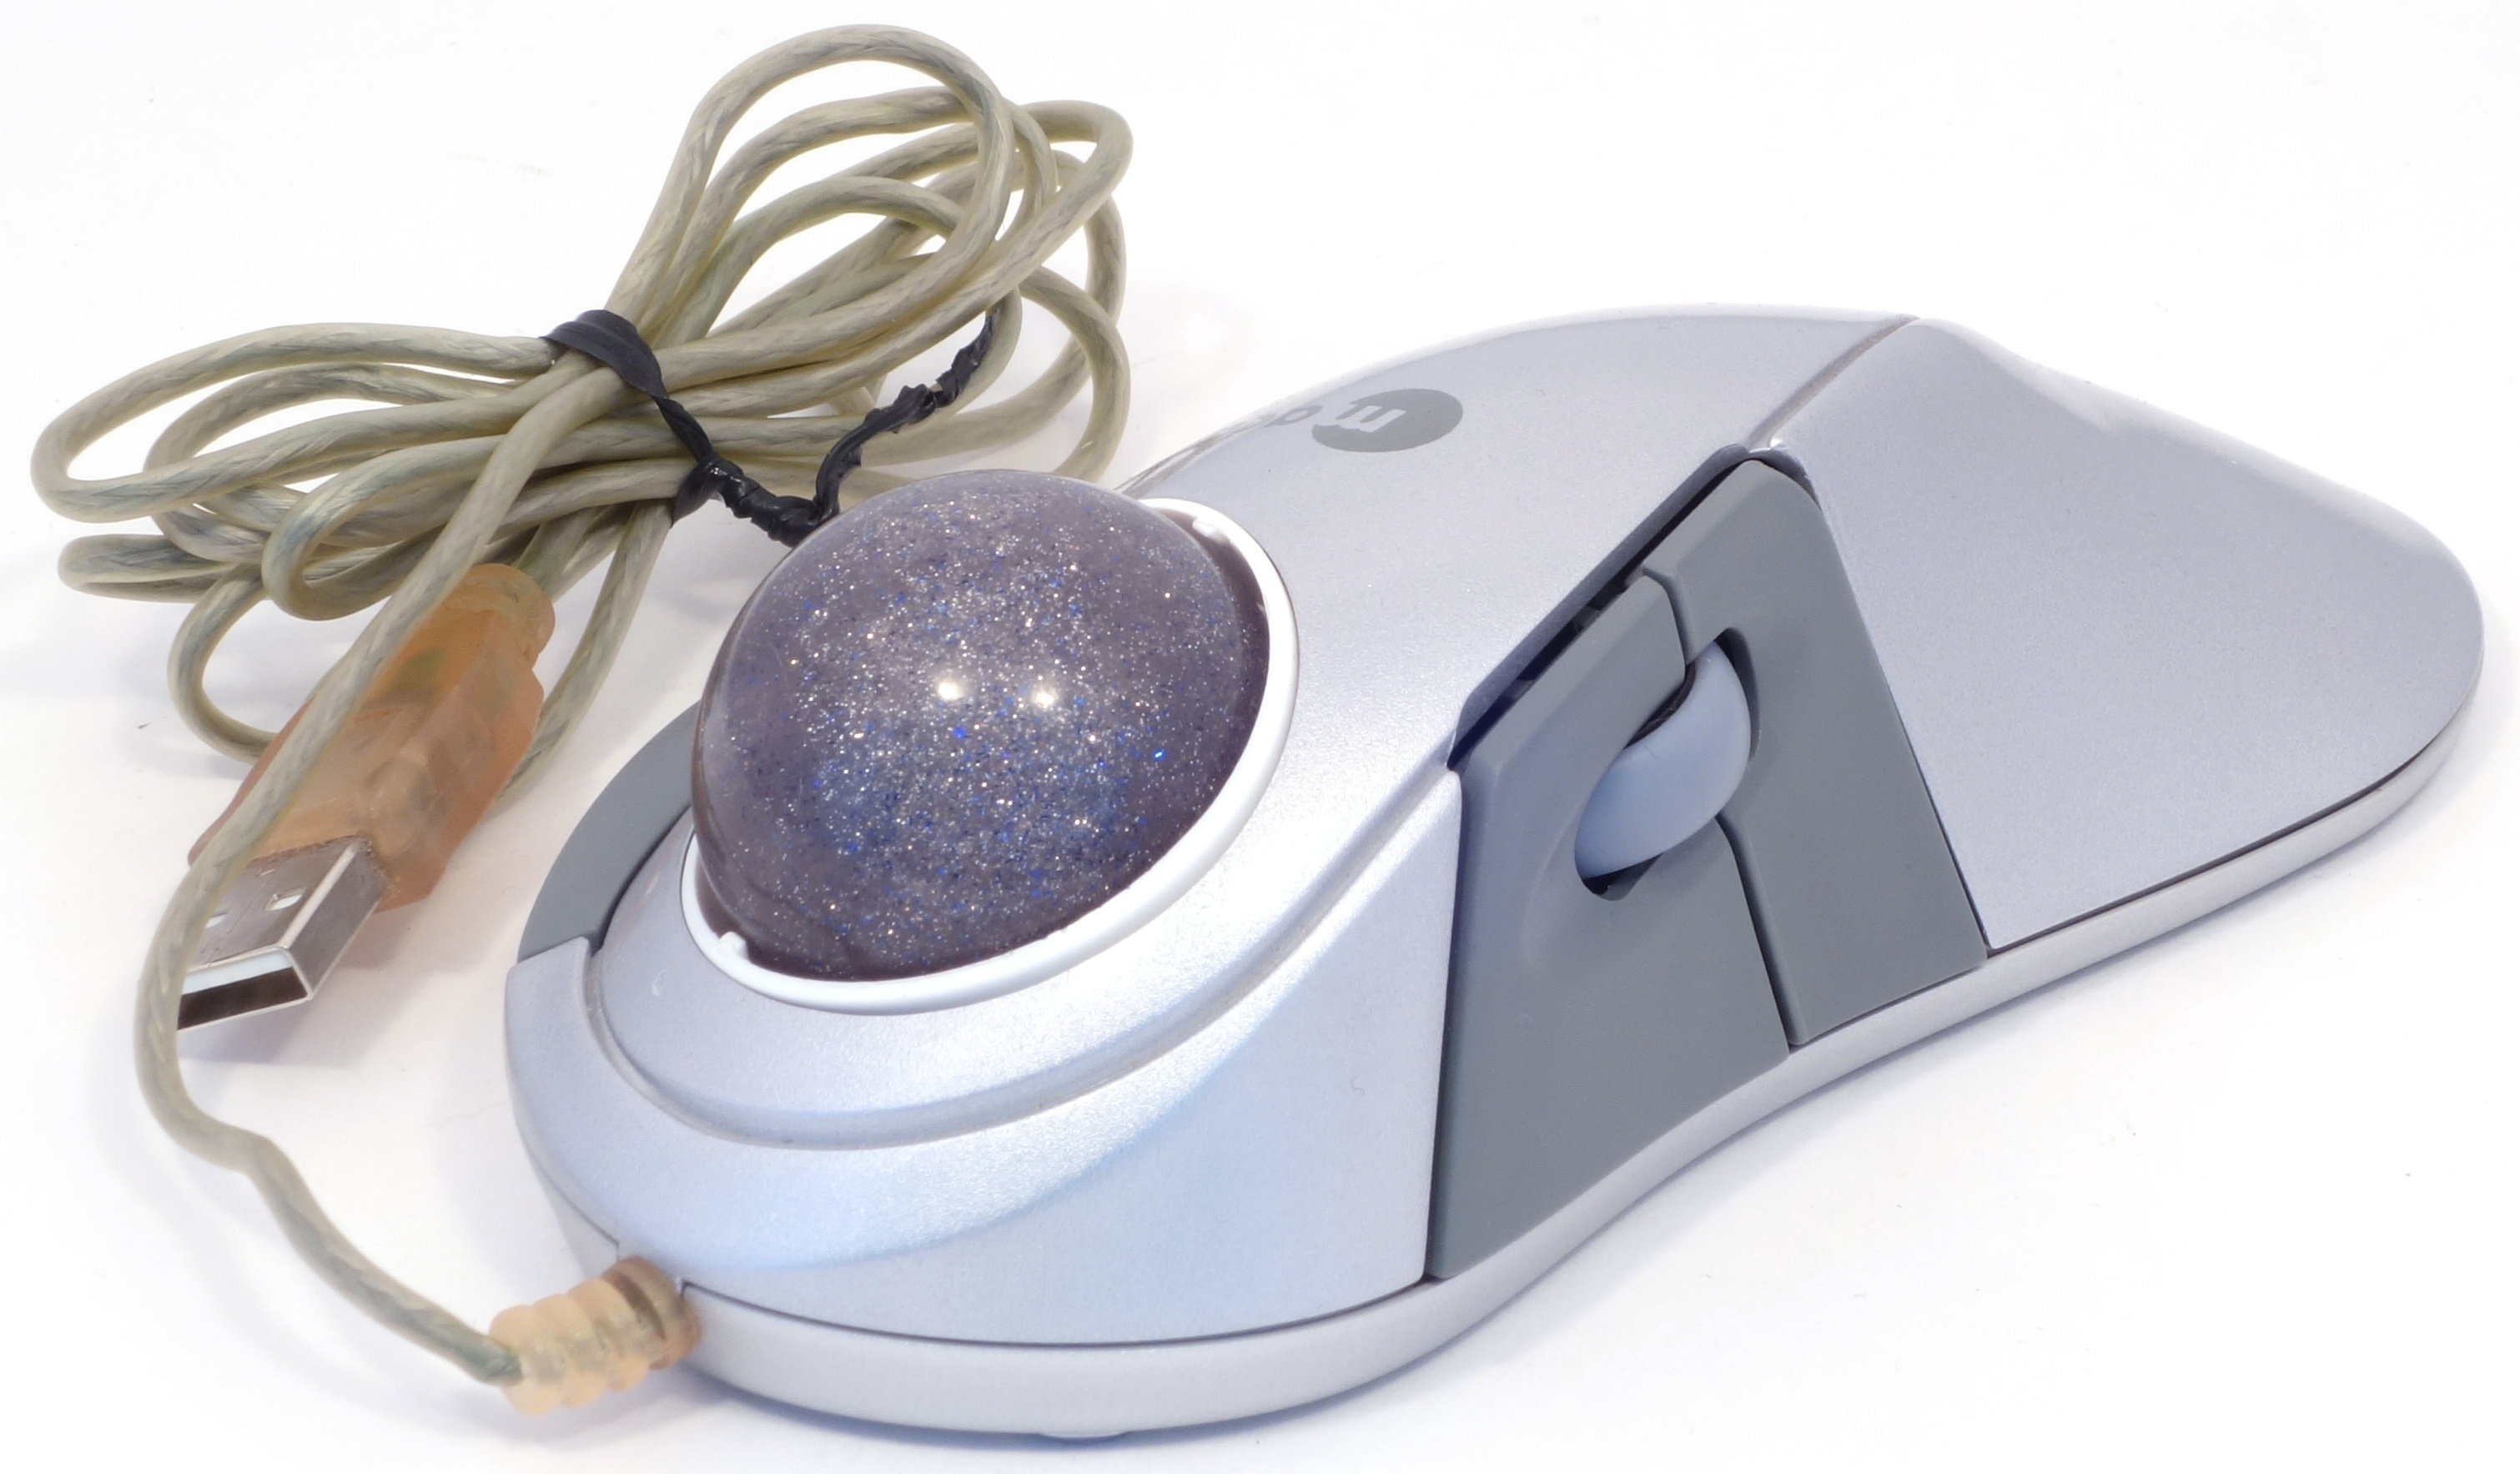
\includegraphics[scale=0.5]{2001_macally_qball/pic_30.jpg}
    \caption{Macally QBALL}
    \label{fig:MacallyQBALLPic}
\end{figure}

A feature of the trackball is a translucent ball with small glittering particles, the so-called ``Glitter Ball'' \cite{site}. At rest, the ball is slightly illuminated by a red LED, and at the moment of rotation, the brightness of the backlight increases \cite{review}, making it easier for the optical sensor to detect the movement of particles contained in the ball.

\begin{figure}[h]
    \centering
    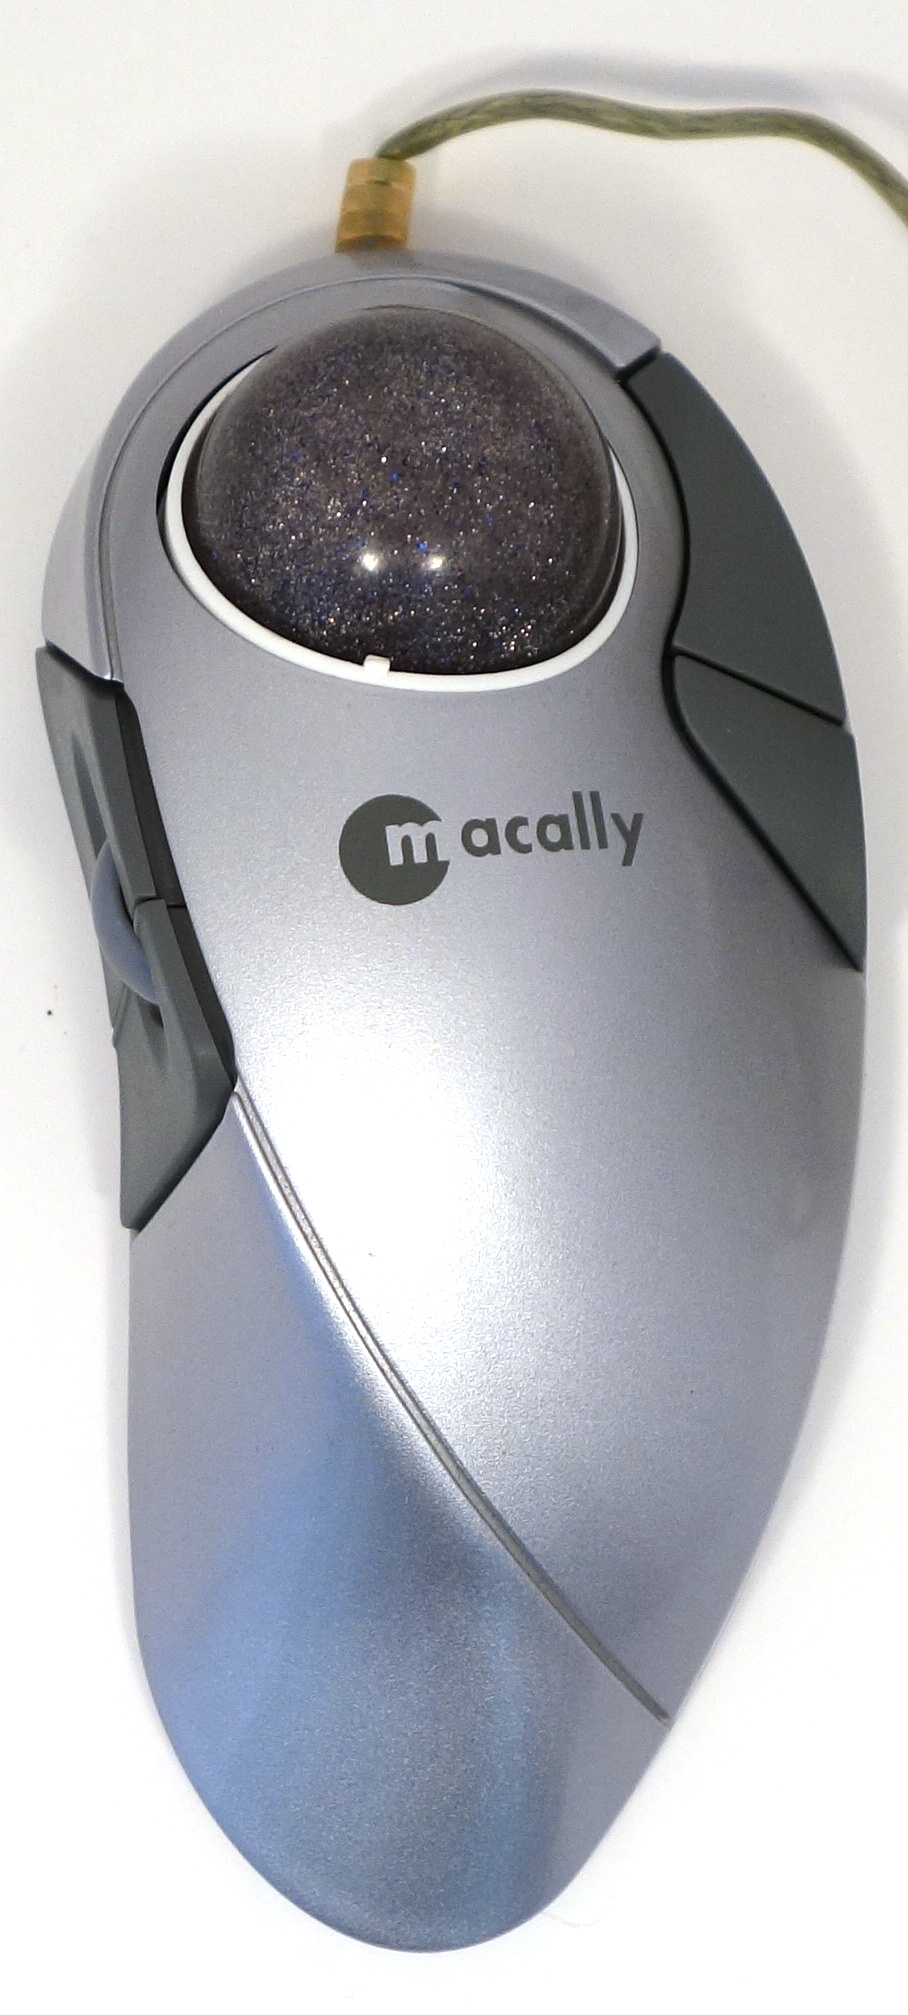
\includegraphics[scale=0.45]{2001_macally_qball/top_30.jpg}
    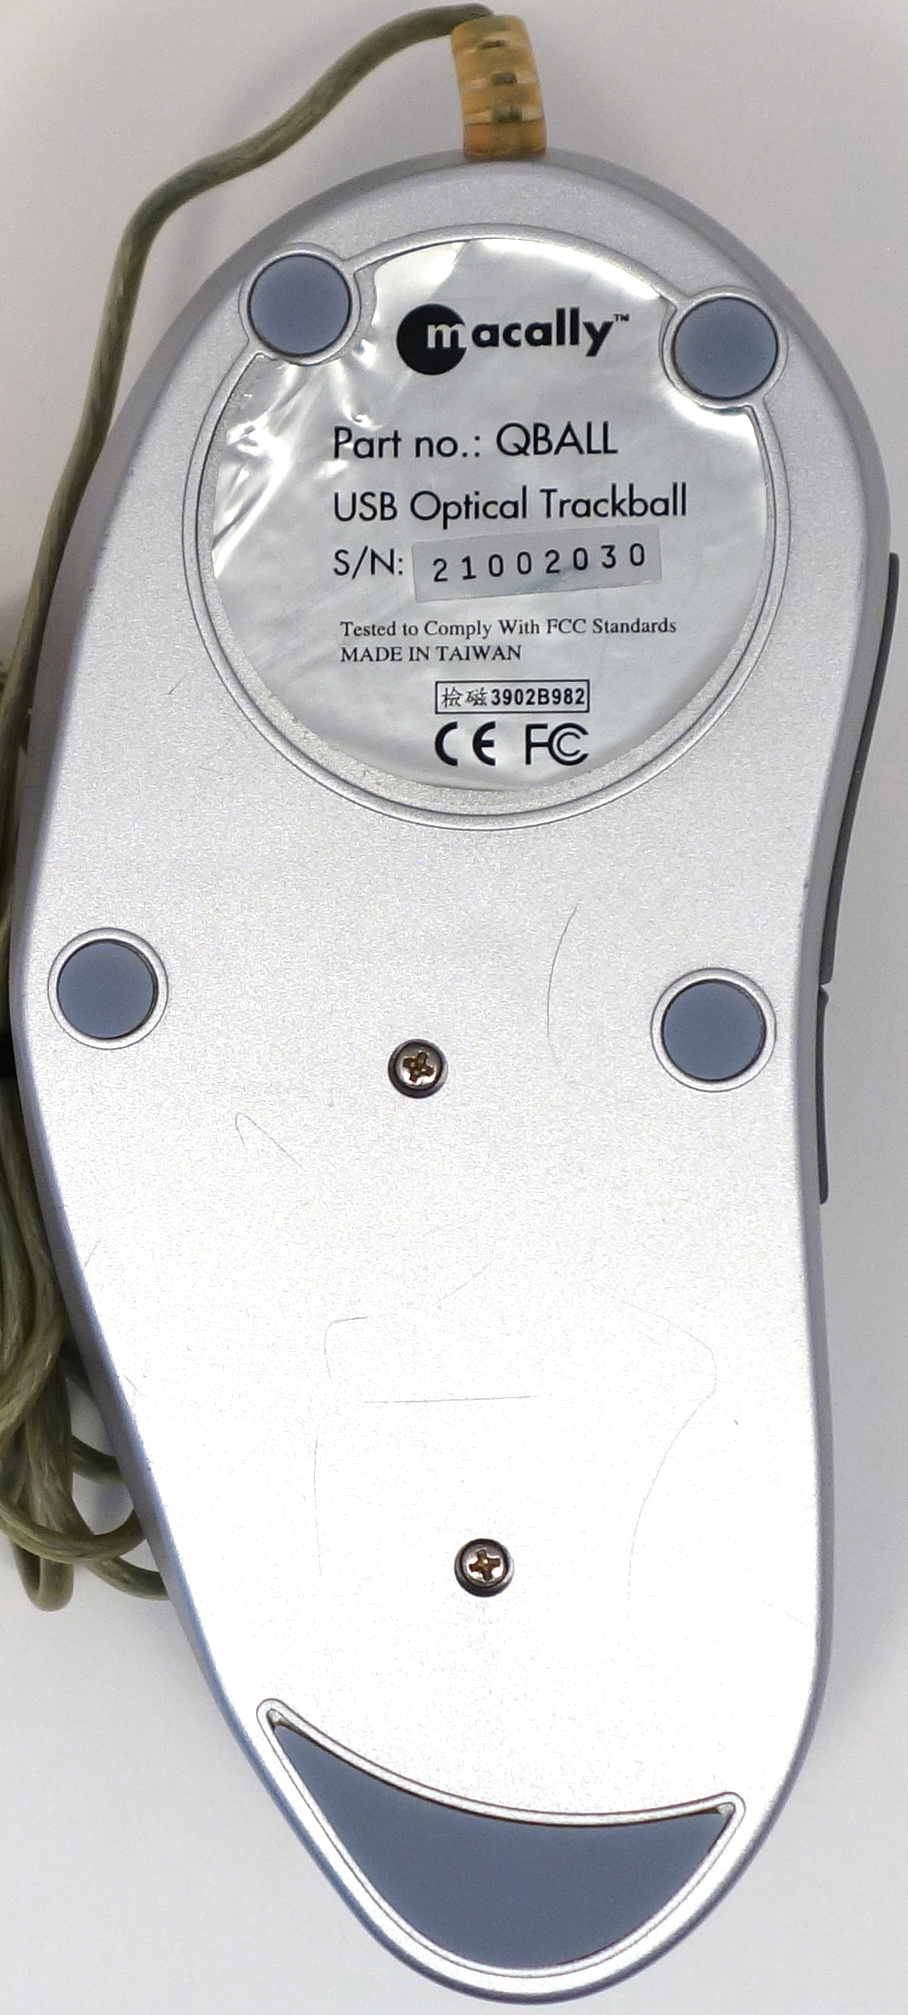
\includegraphics[scale=0.45]{2001_macally_qball/bottom_30.jpg}
    \caption{Macally QBALL, top and bottom views}
    \label{fig:MacallyQBALLTopBottom}
\end{figure}

This trackball has an asymmetrical design with 5 buttons and a scroll wheel (fig. \ref{fig:MacallyQBALLTopBottom}).
The large left and right buttons near the ball are the 1st and 2nd mouse buttons, and the pair of buttons further away from the ball are the 4th and 5th buttons.
The button on the left side of the body is pressed with the thumb to the right, while the button on the right side is pressed with the ring finger. The button combined with the scroll wheel, which performs the traditional role of the 3rd mouse button, is pressed quite hard, which prevents accidental clicks when scrolling.

\begin{figure}[h]
    \centering
    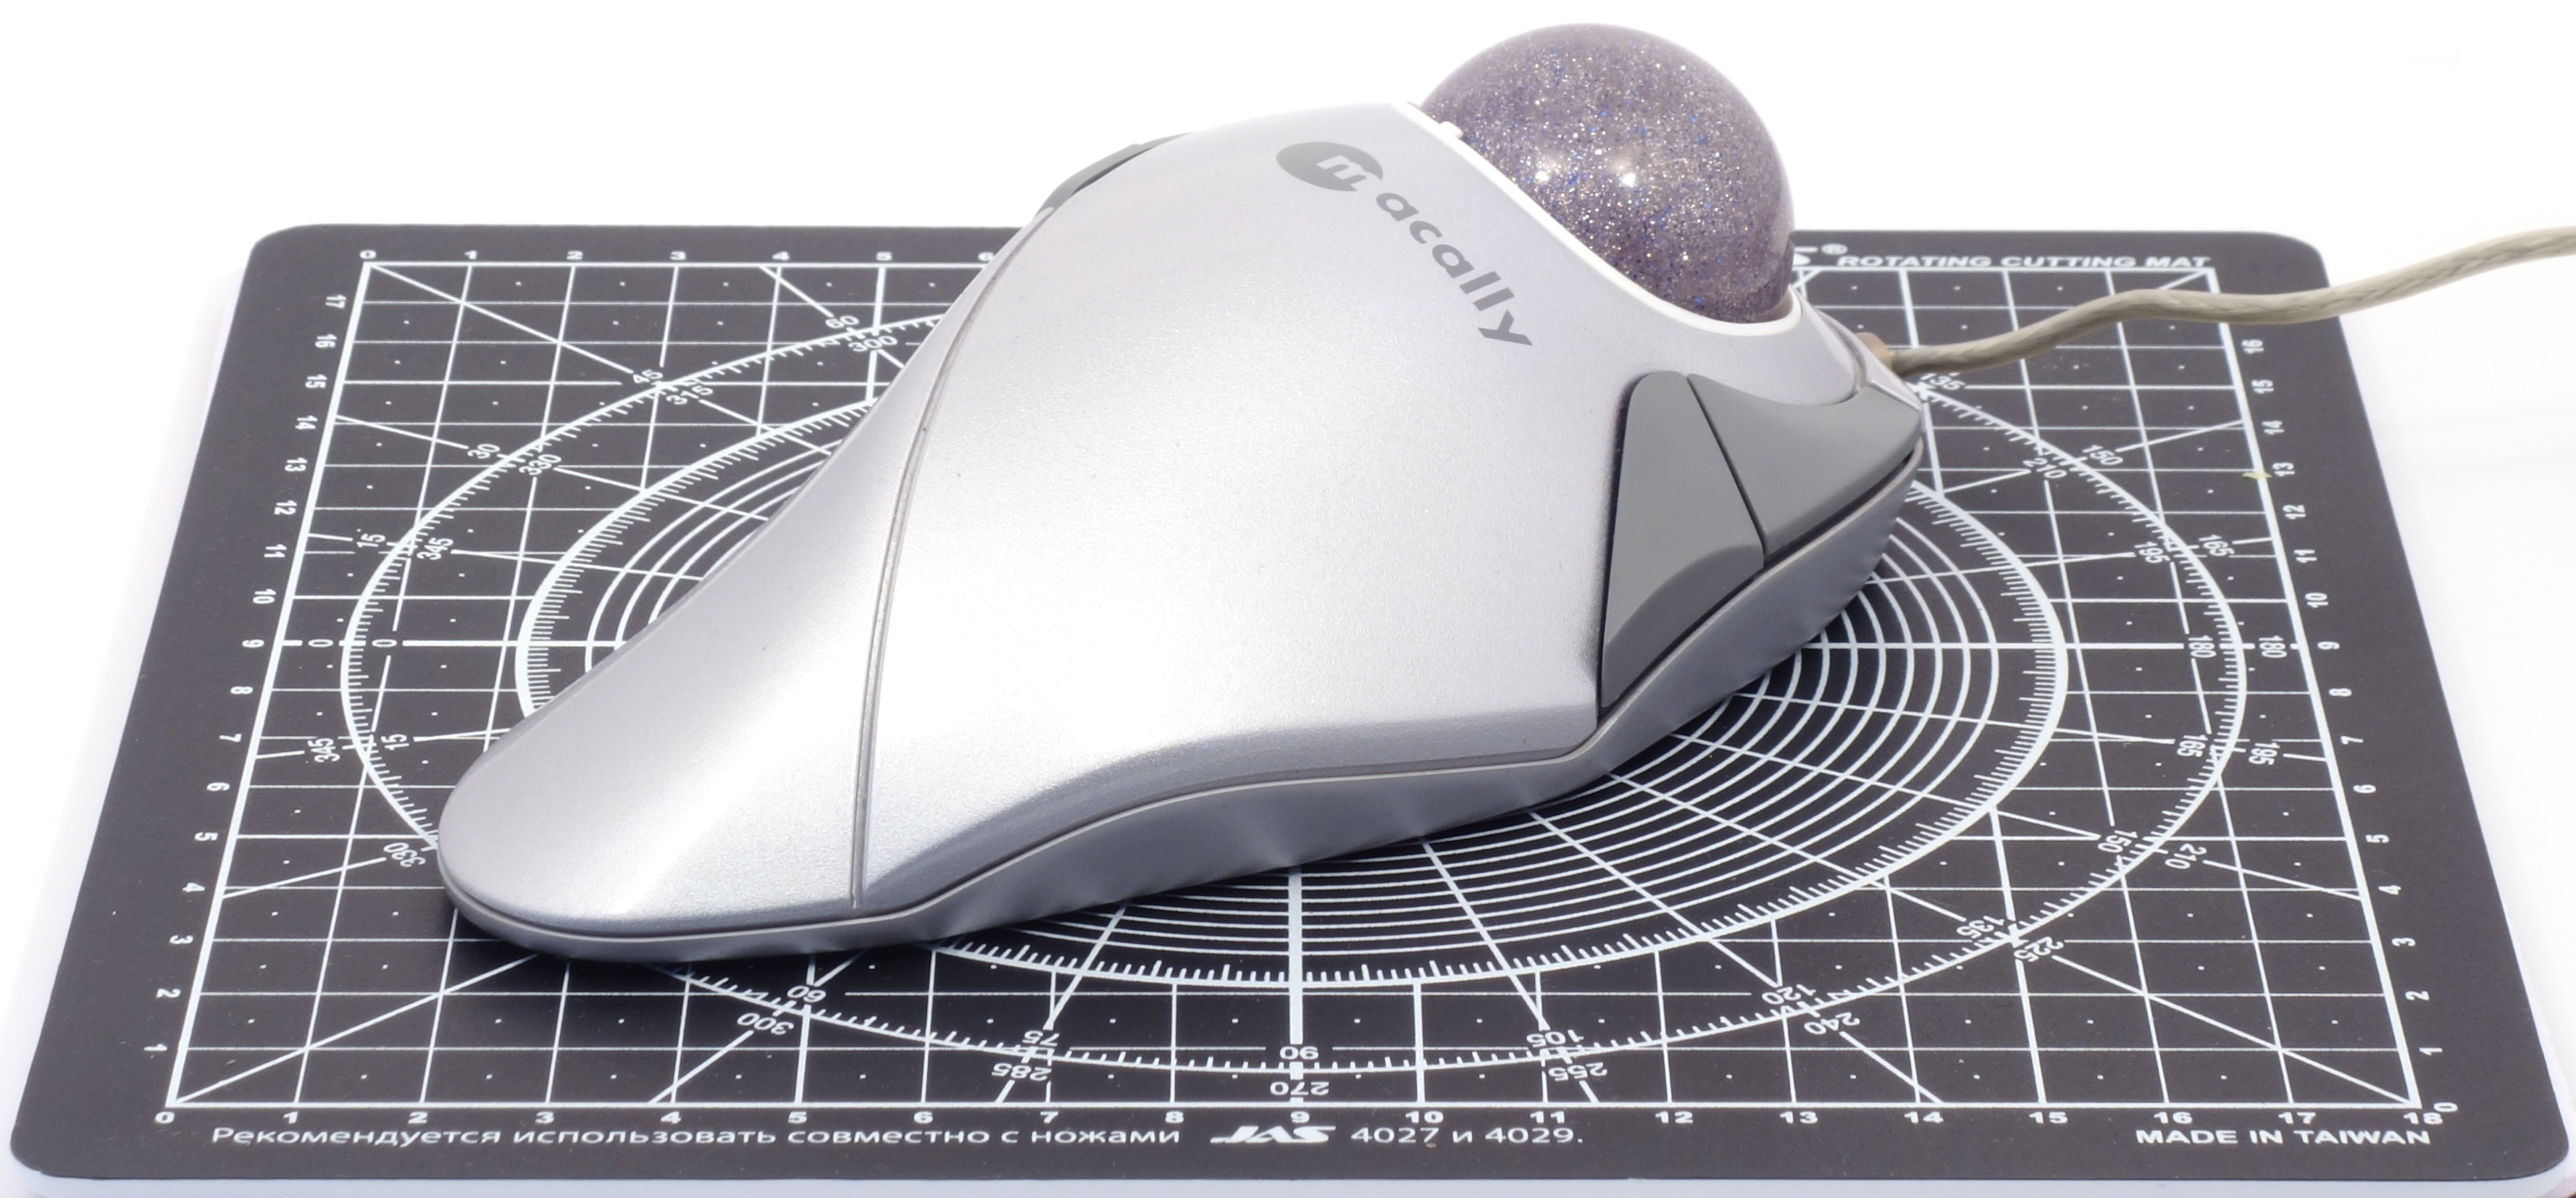
\includegraphics[scale=0.5]{2001_macally_qball/size_30.jpg}
    \caption{Macally QBALL on a graduated pad with a grid step of 1~cm}
    \label{fig:MacallyQBALLSize}
\end{figure}

The QBALL creators for sure were ispired by the Microsoft Trackball Explorer model. There are small changes in shape of the palm rest and in size: QBALL is smaller than the Microsoft trackball (fig. \ref{fig:MacallyQBALLSize}), but in general, the similarity is obvious at a glance.

\begin{figure}[h]
    \centering
    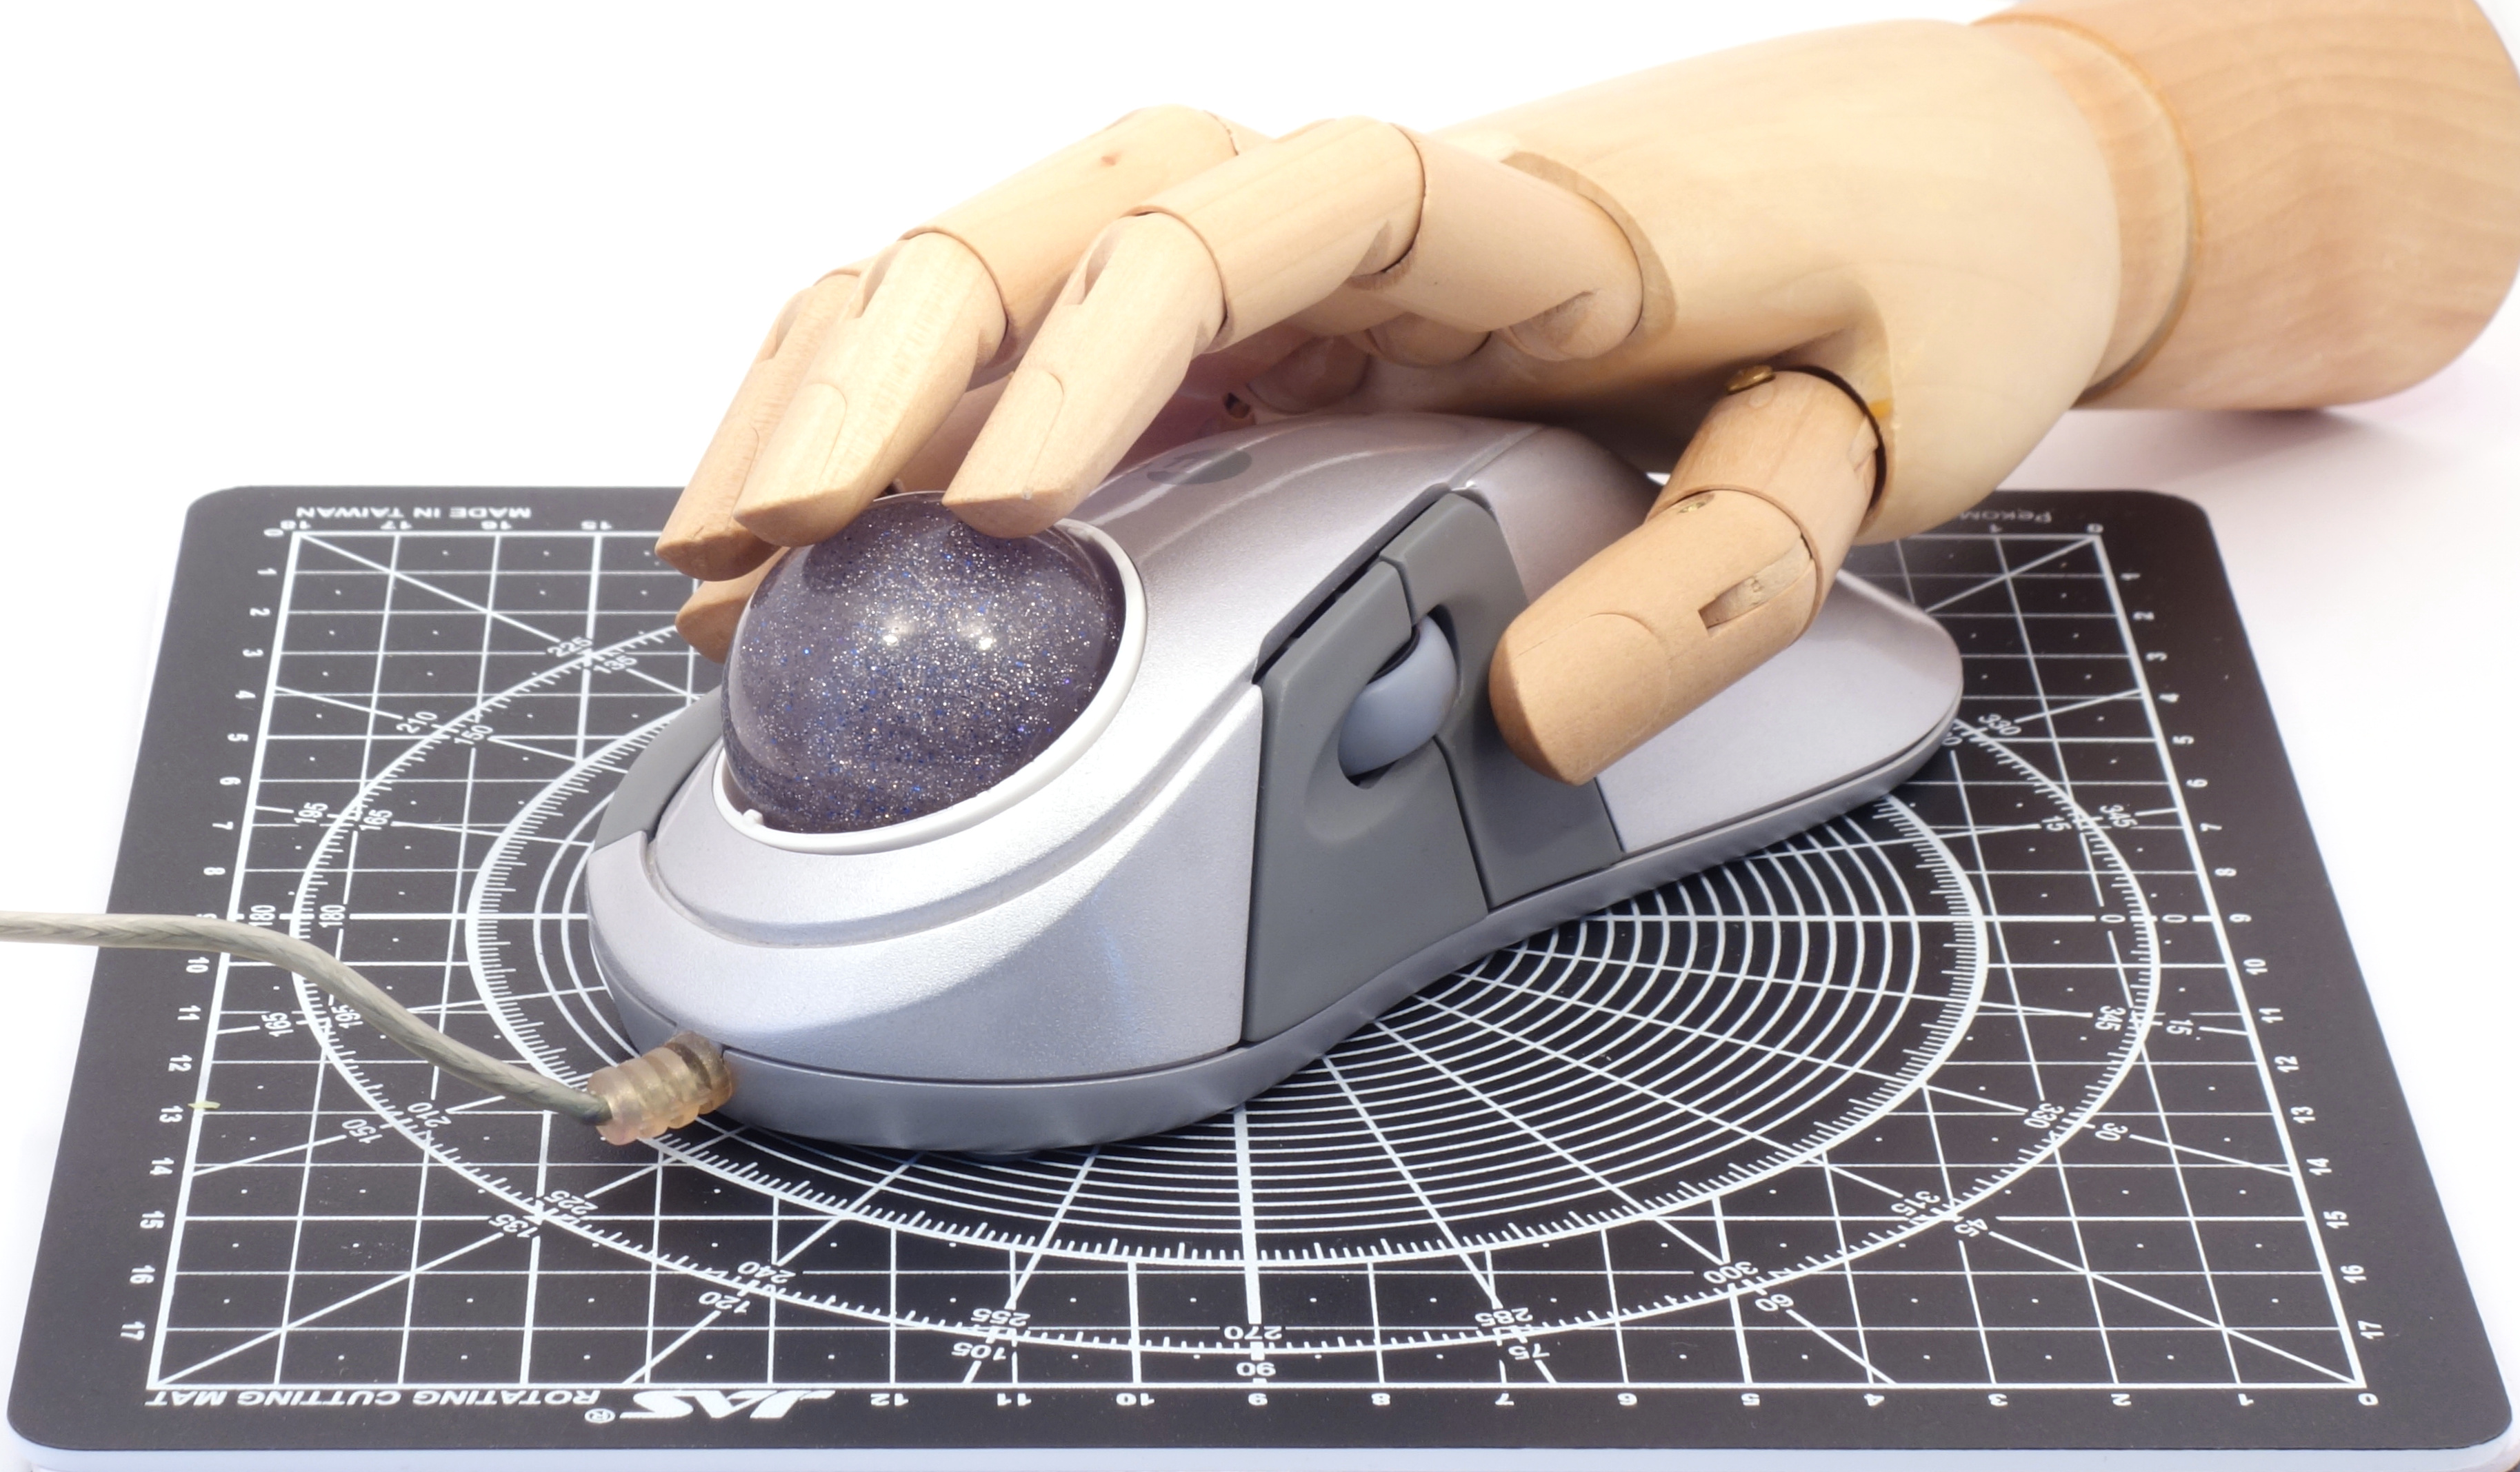
\includegraphics[scale=0.5]{2001_macally_qball/hand_30.jpg}
    \caption{Macally QBALL with a human hand model}
    \label{fig:MacallyQBALLHand}
\end{figure}

In terms of ergonomics, we can note a comfortable body shape and well-placed large buttons (fig. \ref{fig:MacallyQBALLHand}). The asymmetrical shape provides comfortable hand support and a conveniently located scroll wheel, but makes the trackball suitable for right-handers only.

\begin{figure}[h]
    \centering
    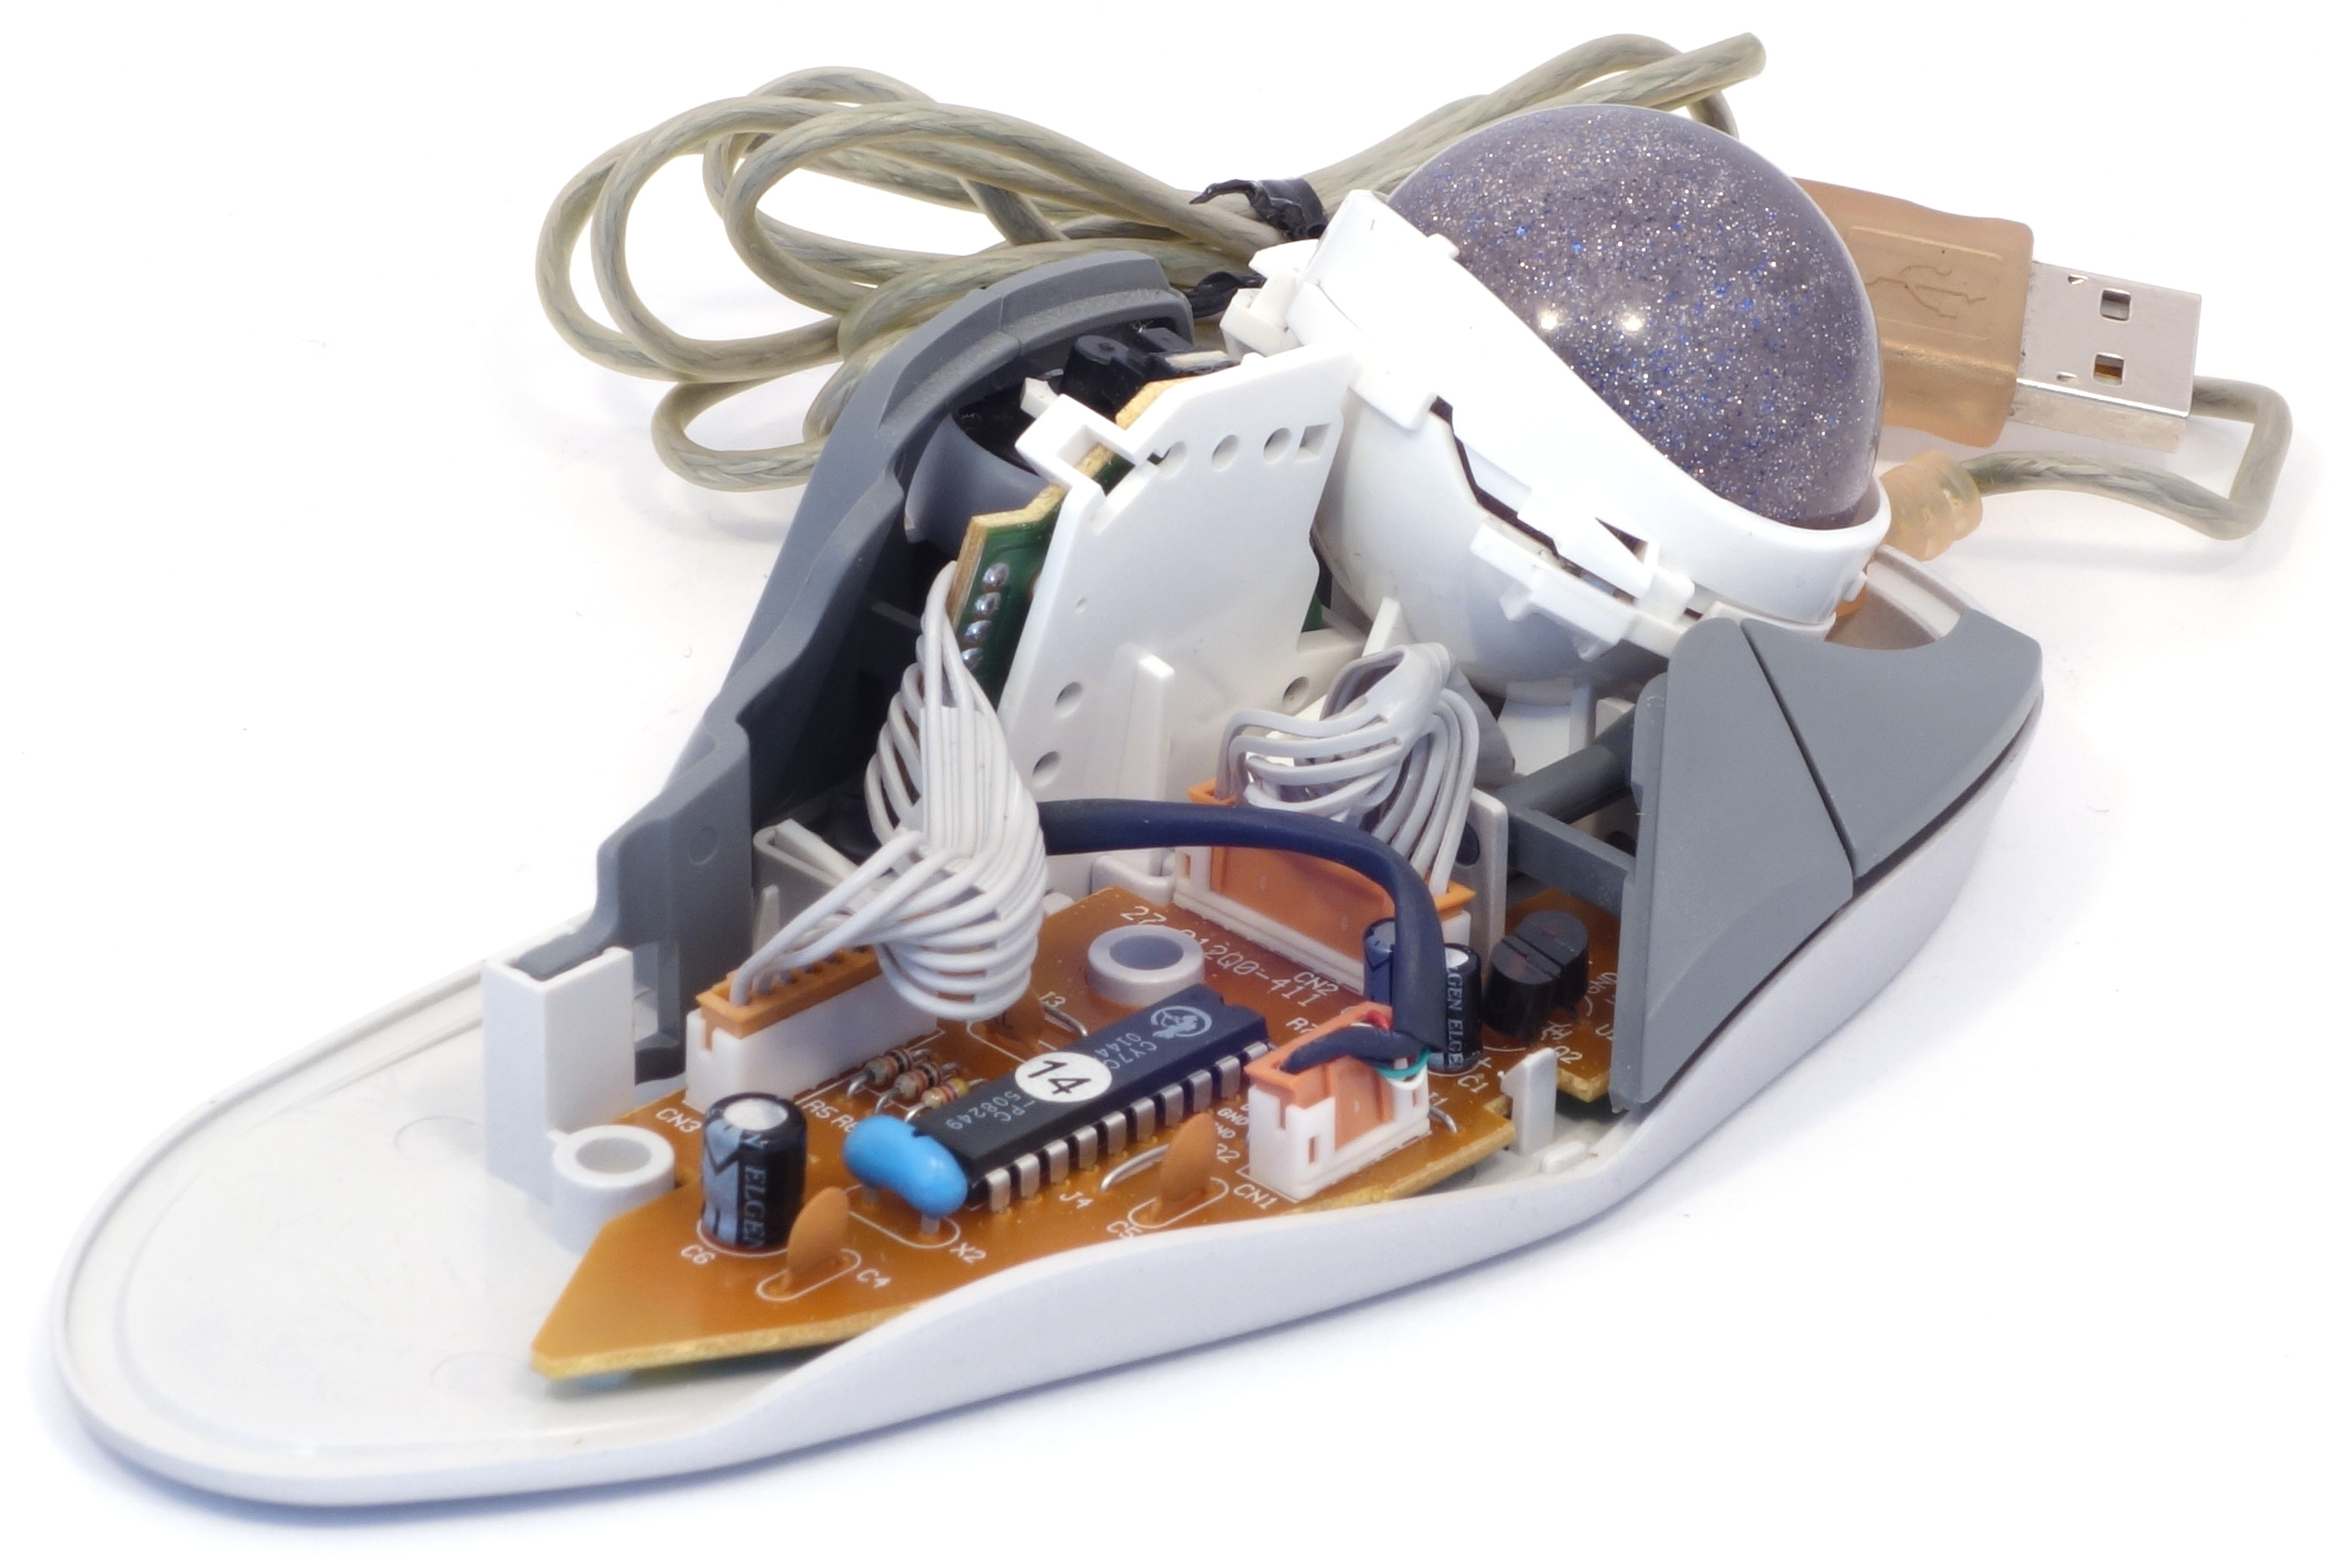
\includegraphics[scale=0.7]{2001_macally_qball/inside_60.jpg}
    \caption{Macally QBALL disassembled}
    \label{fig:MacallyQBALLInside}
\end{figure}

The trackball internals can be seen in the fig. \ref{fig:MacallyQBALLInside}. As you can see, the QBALL is a fully optical trackball. However, the ball rests on metal rollers, which is more typical of optomechanical trackballs (in most cases, the ball of optical trackballs slides on fixed point bearings with low friction).

The \cite{trackballfan} speculates the rolling bearing to be used due to the insufficiently smooth surface of the ball. On the manufacturer's official website \cite{site}, metal support rollers are mentioned as an additional advantage of the model, which ensures smoother movement of the ball and less regular cleaning.

\begin{thebibliography}{9}
\bibitem{site} Products -- USB Optical Trackball for Mac \url{https://web.archive.org/web/20010802210604/http://www.macally.com:80/spec/usb/input_device/qball.html}
\bibitem{trackballfan} Trackball Fan! [in Japanese] \url{http://www.hykw.com/tbfan/reviews/pcgb.shtml}
\bibitem{review} VHJ: Review of the Macally Qball in a WinXP Environment \url{https://vanshardware.com/reviews/2004/07/040712_MacallyQball/040712_MacallyQball.htm}
\end{thebibliography}
\end{document}
